\documentclass[11pt,a4paper]{article}
\usepackage[utf8]{inputenc}
\usepackage[spanish]{babel}
\usepackage{amsmath}
\usepackage{amsfonts}
\usepackage{amssymb}
\usepackage{graphicx}
\usepackage[left=1.2cm,right=1.2cm,top=2cm,bottom=2cm]{geometry}
\date{\small{\today}}
\usepackage{fancyhdr}
\usepackage{afterpage}
\usepackage{titlesec}
\usepackage{float}
\usepackage{gensymb}
\usepackage{xfrac}
\usepackage{tabularx}
\usepackage{multicol}
\usepackage[font=small]{caption}
\usepackage{scrextend}
\usepackage[toc,page]{appendix}
\usepackage{tikz}
\usepackage{tkz-euclide}
\usepackage[siunitx,americanvoltages,fulldiodes]{circuitikz}
\usepackage{stackengine}
\usepackage{mathtools}
\usepackage{hyperref}
\DeclarePairedDelimiter\abs{\lvert}{\rvert}%
\DeclarePairedDelimiter\norm{\lVert}{\rVert}%
\usetikzlibrary{arrows}
\usepackage{caption}

\renewcommand\appendixpagename{Apéndices}
\renewcommand\appendixname{Apéndice}

\DeclareMathOperator{\arctantwo}{arctan2}

\titleformat{\section}{\Large\bfseries}{}{0em}{}[]
\titleformat{\subsection}{\large\bfseries}{}{0em}{}[]
\titleformat{\subsubsection}{\bfseries}{}{0em}{}[]
\titleformat{\chapter}{\large\bfseries}{}{0em}{}[]


\setlength\parindent{0pt}


\begin{document}
\title{Adaptación de Impedancia en Guía de Onda Rectangular}
	\LARGE{\textsc{Laboratorio II}}\\
	\Large{Adaptación de Impedancia en Guía de Onda Rectangular}\\
\begin{large}
\small\textsc{Bercic, Jerónimo}\\
\small\textsc{Roqueta, Matías Daniel}\\
\small{Instituto Balseiro, Centro Atómico Bariloche, Comisión Nacional de Energía Atómica}\\
\end{large}
\setcounter{page}{1}

\lhead{Laboratorio II}%Materia
\rhead{Adaptación de Impedancia en Guía de Onda Rectangular}%Título 
\chead{}

\lfoot{J. Bercic, M. Roqueta}
\cfoot{Instituto Balseiro} 
\rfoot{\thepage} 
\renewcommand{\headrulewidth}{0.4pt} 
\renewcommand{\footrulewidth}{0.4pt} 
\pagestyle{fancy}

\hrule
\normalsize
\section{Resumen}
Se midió la frecuencia de trabajo de una fuente de microondas electromagnéticas y su longitud de ondas, resultando en $f=(10.53\pm0.05)$ GHz y $\lambda_g=(3.97\pm)$ cm, respectivamente. También se caracterizó una guía de ondas para distintos planos de carga. Luego, se verificó que la señal transmitida por la guía aumenta si ésta se encuentra con la impedancia adaptada. 

\begin{multicols}{2}
\section{Introducción}
Una guía de ondas electromagnéticas es un dispositivo que se utiliza para restringir la energía de una onda, y que ésta sea propagada en una dirección deseada. De esta manera se puede aprovechar dicha energía de manera más eficiente. Su utilidad es evidente, por ejemplo, en la fabricación de antenas, donde se busca que la propagación sea en una dirección específica y que las pérdidas de información sean mínimas. En la Figura \ref{fig:guia} se muestra una guía de ondas electromagnéticas rectangular.
\begin{figure}[H]
    \centering
    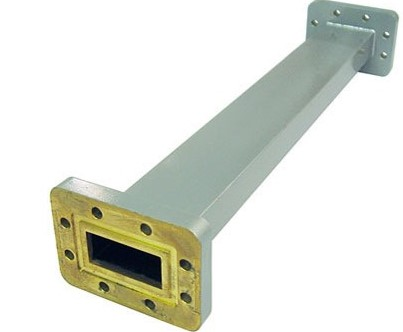
\includegraphics[scale=0.6]{Images/Imagen1.jpg}
    \caption{Guía de ondas electromagnéticas rectangular.}
    \label{fig:guia}
\end{figure}
Dentro del contexto de éste tipo de guía de ondas, se encuentran los que se conocen como modos TE$_{mn}$ (Transverse Electric Field) y TM$_{mn}$ (Transverse Magnetic Field), que se refieren a si la onda transversal a la dirección de propagación es la eléctrica o la magnética, respectivamente, $m$ es el número de medias-ondas a lo largo de la guía, y $n$ es el número de medias-ondas a lo alto de la guía. En la Figura \ref{fig:te10} se presenta un esquema de una guía de ondas cuyo modo es el TE$_{10}$.
\begin{figure}[H]
    \centering
    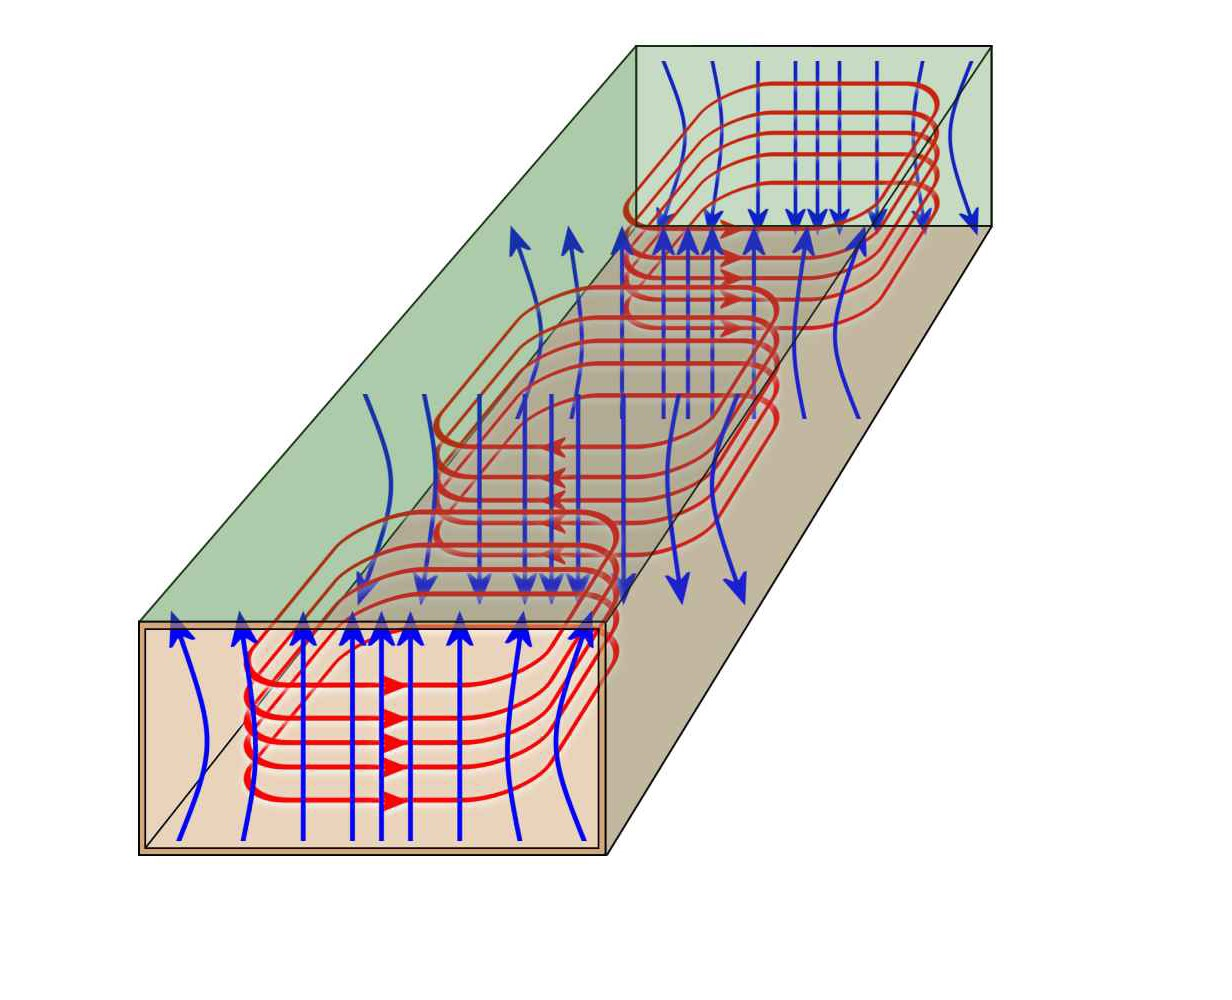
\includegraphics[scale=0.15]{Images/TE10.jpg}
    \caption{Guía de ondas electromagnéticas con modo TE$_{10}$.}
    \label{fig:te10}
\end{figure}
Estos modos de propagación dependerán tanto de las dimensiones de la guía, así como de la frecuencia de la onda propagada. \\ \\
Para poder caracterizar la guía de ondas, se puede pensar en ella como una línea de transmisión, o sea, una cascada de cuadripolos (Figura \ref{fig:cuadri}) distribuidos a lo largo de la línea.
\begin{figure}[H]
\centering
\begin{tikzpicture}[scale=0.75]
\draw (1,3) to [L, l_=$L\:dz$] (-2,3);
\draw (1,3) to [C, l_=$C$] (1,1);
\draw[ultra thin, fill=pink,fill opacity=0.15] (-3,0.25) rectangle (2,3.8);
\draw[->] (-2,1) -- (3,1);
\draw[->] (-2,3) -- (3,3);
\draw (-4,1) -- (-2,1);
\draw (-4,3) -- (-2,3);
\draw (-2,3) -- (-2,1);
\node at (-7,1) { };
\draw[->] (-5.5,3) -- node[above] {$i(z,t)$} (-4.2,3);
\draw[->] (3.2,3) -- node[above] {$i(z+dz,t)$} (4.4,3);
\draw[->] (-4.2, 1.2) -- node[left] {$v(z,t)$} (-4.2,2.7);
\draw[->] (3.2, 1.2) -- node[right] {$v(z+dz,t)$} (3.2,2.7);
\end{tikzpicture}
\caption{Cuadripolo a disponer en cascada, que caracteriza a una línea de transmisión.}\label{fig:cuadri}
\end{figure}



Al igual que una línea de transmisión, las guías de ondas cuentan con una impedancia característica $Z_0$. Para la guía, se puede calcular sabiendo la frecuencia $f$ a la que se propaga la onda, de la siguiente forma
\begin{equation}
    Z_0=\frac{Z_\text{vacío}}{\lambda_\text{vacío}}=Z_\text{vacío}\frac{f}{c}\lambda_g
\end{equation}
Donde $Z_\text{vacío}$ es la impedancia característica del vacío, igual a $376.6$ $\Omega$, $\lambda_\text{vacío}$ es la longitud de la onda propagada si ésta se propagase en el vacío, y $c$ es la velocidad de la luz, y $\lambda_g$ la longitud de la onda dentro de la guía.\\ \\
Sabiendo la impedancia característica de la guía de ondas, se puede adaptar a la impedancia  $Z_\text{L}$ del plano de carga, y así poder aprovechar de manera más eficiente la energía transmitida. Éste será el caso si $Z_0$ es igual a $Z_\text{L}$. Para saber si la guía está adaptada se utiliza el \textbf{coeficiente de reflexión} $\Gamma$,
\begin{equation}\label{eq:gamma}
    \Gamma = \frac{Z_\text{L}-Z_0}{Z_\text{L}+Z_0}
\end{equation}
el cual vale $\Gamma = -1$ para un corto circuito, $\Gamma = 1$ para un circuito abierto, y $\Gamma = 0$ para la guía adaptada.\\ \\ 
Otra forma de verificar si la guía está adaptada, es analizando la onda estacionaria que se forma debido a la reflexión de la onda en el plano de carga (Figura 4).
\begin{center}
    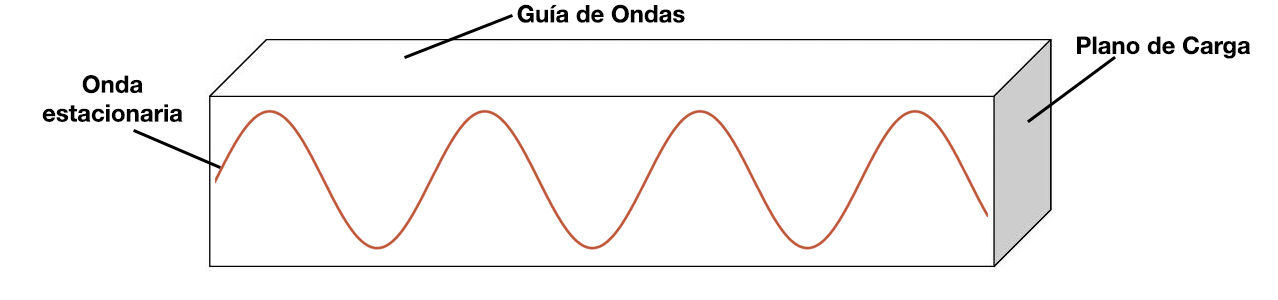
\includegraphics[scale=0.28]{Images/Para el informe.jpg} \\
    \textbf{Figura 4}: Onda estacionara formada en la guía debido a la reflexión en el plano de carga. 
\end{center}
Para ello se define el ROE (razón de onda estacionaria) como
\begin{equation}
    \text{ROE} = \frac{1+\abs{\Gamma}}{1-\abs{\Gamma}}
\end{equation}
Este número también se puede calcular haciendo el cociente entre las amplitudes máxima y mínima de la onda estacionaria, y tiene un rango de 
$$
1<\text{ROE} < \infty
$$
Cuanto se quiere adaptar la guía, el ROE debe tender a 1. \\ \\
En este laboratorio, se busca medir las propiedades de la onda estacionaria que se forma bajo distintas condiciones del plano de carga. Además, se busca adaptar la impedancia a la vez que se mide la señal transmitida. 
\subsection{Adaptación de Impedancia}

Suponer que se cuenta con una una línea de transmisión semi-infinita, cuya impedancia del plano de carga normalizada es $z_L$.
De la ecuación \ref{eq:gamma} se valida que la impedancia está adaptada cuando $Z_L = Z_0 \longrightarrow z_L = 1$.\\

Esta impedancia de carga normalizada, varía en función de la distancia $x$ al plano de carga según la siguiente expresión,
\begin{equation*}
    z(x) = \frac{Z_L + j Z_0\tan(kx)}{Z_0 + j Z_L\tan(kx)}
\end{equation*}\ref{eq:zx}
O bien su expresión equivalente
\begin{equation*}
    z(x) = \frac{1 + \Gamma e^{-j2kx}}{1 - \Gamma e^{-j2kx}}
\end{equation*}
donde $k=\frac{2\pi}{\lambda_g}$ es el número de onda, y $j=\sqrt{-1}$. \\ \\
Es equivalente trabajar con la admitancia normalizada en función de la distancia $y(x)$,
\begin{equation*}
    y(x) = \frac{1}{z(x)} = \frac{1 - \Gamma e^{-j2kx}}{1 + \Gamma e^{-j2kx}}
\end{equation*}
Esta expresión permite calcular la admitancia de carga de dos guías en paralelo,
\begin{figure}[H]
    \centering
    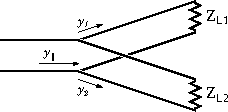
\includegraphics[width=0.7\linewidth]{Images/guiapll.pdf}
    \caption{Paralelo de dos guías de onda. La admitancia de entrada del paralelo cumple $y_\parallel = y_1+y_2$.}
    \label{fig:pll}
\end{figure}

El método de adaptación de impedancia con stub en paralelo consiste en:
\begin{enumerate}
    \item Encontrar en la guía un punto $x = \ell$ tal que la resistencia en $\ell$ esté normalizada, o sea que $y_1(\ell)=1+jb$.
    \item Colocar en $x=\ell$ una admitancia en paralelo puramente reactiva, de valor $y_a = -jb$.
\end{enumerate}

De esta forma se genera a la entrada del paralelo un nuevo plano de carga con admitancia adaptada 
$$y_L' = y(\ell) + y_a = 1$$

Los métodos para encontrar los valores de $\ell$ y $y_a$ consisten en métodos analíticos, numéricos, o usando el diagrama de Smith.


\section{Método Experimental}

Primero se determina la frecuencia $f$ de emisión del diodo emisor. Luego se construye una línea de transmisión con guía de onda rectangular, conectando en cascada los siguientes elementos, como se ilustra en la Figura \ref{fig:arr1}.
\begin{multicols}{2}
    \begin{labeling}{III} 
        \item [I] Emisor Diodo Gunn
        \item [II] Aislador
        \item [III] Atenuador 3 dB
        \item [IV] Cavidad Resonante
        \item [V] Antena Detectora
        \item [VI] Cortocircuito Móvil
    \end{labeling}        
\end{multicols}
\begin{figure}[H]
    \centering
    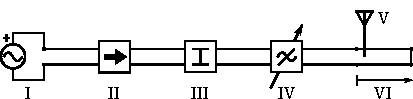
\includegraphics[width=\linewidth]{Images/arreglo1.pdf}
    \caption{Línea de transmisión para medir frecuencia de emisión. La cavidad resonante actúa como filtro, absorbiendo su frecuencia de resonancia y dejando pasar otras frecuencias.}
    \label{fig:arr1}
\end{figure}
Se ajusta el cortocircuito móvil hasta detectar un máximo de onda estacionaria con la antena detectora, y se procede a ajustar la frecuencia de resonancia de la cavidad hasta que esta coincida con la frecuencia de emisión del diodo Gunn.\\ \\
Conociendo la frecuencia de operación del emisor, se procede a caracterizar la longitud de onda $\lambda_g$ dentro de la guía y su impedancia característica $Z_0$. 
\begin{figure}[H]
    \centering
    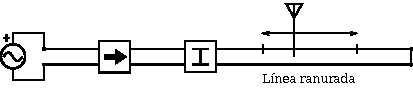
\includegraphics[width=\linewidth]{Images/arreglo2.pdf}
    \caption{Linea de transmisión para medir longitud de onda. La terminación en cortocircuito provoca una onda estacionaria en la guía, la onda estacionaria se mide con una antena detectora en una línea ranurada.}
    \label{fig:arr2}
\end{figure}

Una vez conocidas $\lambda_g$ y $Z_0$, se puede proceder a adaptar impedancias. Se costruye la línea de transmisión correspondiente a la Figura \ref{fig:arr4}.

\begin{figure}[H]
    \centering
    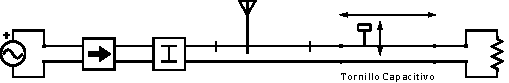
\includegraphics[width=\linewidth]{Images/arreglo4.pdf}
    \caption{Sistema de adaptación de impedancias para una impedancia de carga $Z_L$, un tornillo capacitivo actúa como stub en paralelo.}
    \label{fig:arr4}
\end{figure}

Se sigue el siguiente procedimiento para la adapatación de impedancia

\begin{enumerate}
    \item Se mide la onda estacionaria con $Z_L$ en cortocircuito, referenciando el plano de carga a un mínimo de onda estacionaria.
    \item Se cambia $Z_L$ por una impedancia arbitraria y se mide la onda estacionaria. Se calculan la ROE y el desplazamiento $\delta$ del plano de carga.
    \item Usando la ROE y el desplazamiento del plano de carga, se calcula la posición del adaptado $\ell$, la profundidad $s$ con que éste debe ser introducido a la guía, y su admitancia $y_a$. 
    Estos cálculos se realizan con el diagrama de Smith\footnote{Apéndice 1} y numéricamente con un script Python\footnote{Apéndice 2}.
    \item Se ajusta la posición y admitancia del adaptador, se mide la onda estacionaria validando la disminución de la ROE ante impedancia adaptada.
\end{enumerate}

Este método de adaptación de impedancia se utiliza para adaptar un sistema de comunicaciones transmisor-receptor, representado en la Figura \ref{fig:sistema}

\begin{figure}[H]
    \centering
    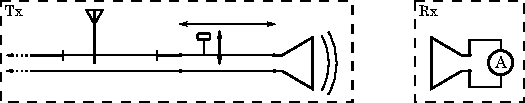
\includegraphics[width=\linewidth]{Images/sistema.pdf}
    \caption{Sistema transmisor-receptor.
    \texttt{Tx:} línea de la figura \ref{fig:arr4} con antena de bocina en $Z_L$. 
    \texttt{Rx:} detector de señal adaptado con una antena de bocina.}
    \label{fig:sistema}
\end{figure}

El sistema se adapta con el siguiente procedimiento
\begin{enumerate}
    \item Se retira el módulo Rx y se mide la ROE, validando que la antena de bocina adapta la impedancia de la guía a la impedancia del espacio libre.
    \item Se ubica el módulo Rx a 10 cm del módulo Tx. Se mide la ROE, observando el incremento de la misma respecto a la medición anterior.
    \item Se realiza el procedimiento de adaptación de impedancia en presencia del módulo Rx.
\end{enumerate}

Se registra la intensidad de señal medida por Rx ant

\section{Resultados}
Para la frecuencia de trabajo de la fuente, se obtuvo un valor de 
$$
f = (10.53 \pm 0.05) \text{ GHz}
$$
que es indistinguible con el valor provisto por el fabricante $f_\text{f}$, que corresponde a $f_\text{f}=10.5$ GHz. \\ \\
La longitud de onda resultó en
$$
\lambda_\text{g} = (3.97 \pm ?) \text{ cm} 
$$
Y la impedancia característica, de la ecuación (1),
$$
Z_0 = (525.6 \pm ?) \text{ } \Omega
$$
Para la medición en cortocircuito (que se consigue colocando una placa de cobre en el plano de carga), se muestra el perfil de la onda en la Figura \ref{fig:cortocir}, 
\begin{figure}[H]
    \centering
    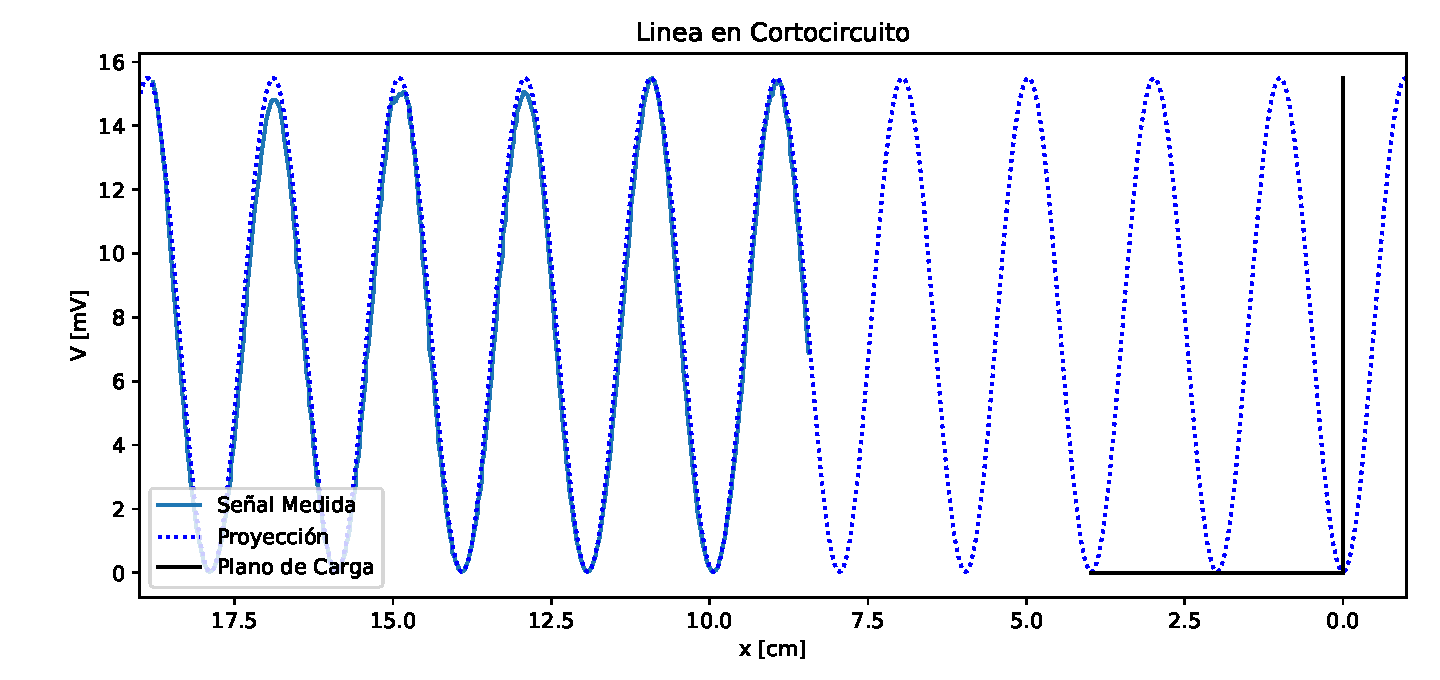
\includegraphics[width=\linewidth]{Images/lineacc.pdf}
    \caption{Perfil de la onda para el caso en que el plano de carga es una placa de cobre. En azul continuo se muestra la curva de los datos obtenidos, en azul punteada, la continuación analítica de la función. La línea negra vertical representa la posición del plano de carga.}
    \label{fig:cortocir}
\end{figure}
Se obtuvo, para este caso, un ROE de
$$
\text{ROE} = 455\pm?
$$
Luego de reemplazar la placa por la antena de bocina en el plano de carga como se muestra en la Figura \ref{fig:sistema}, se obtuvo el siguiente perfil de onda (Figura \ref{fig:bocina}),
\begin{figure}[H]
    \centering
    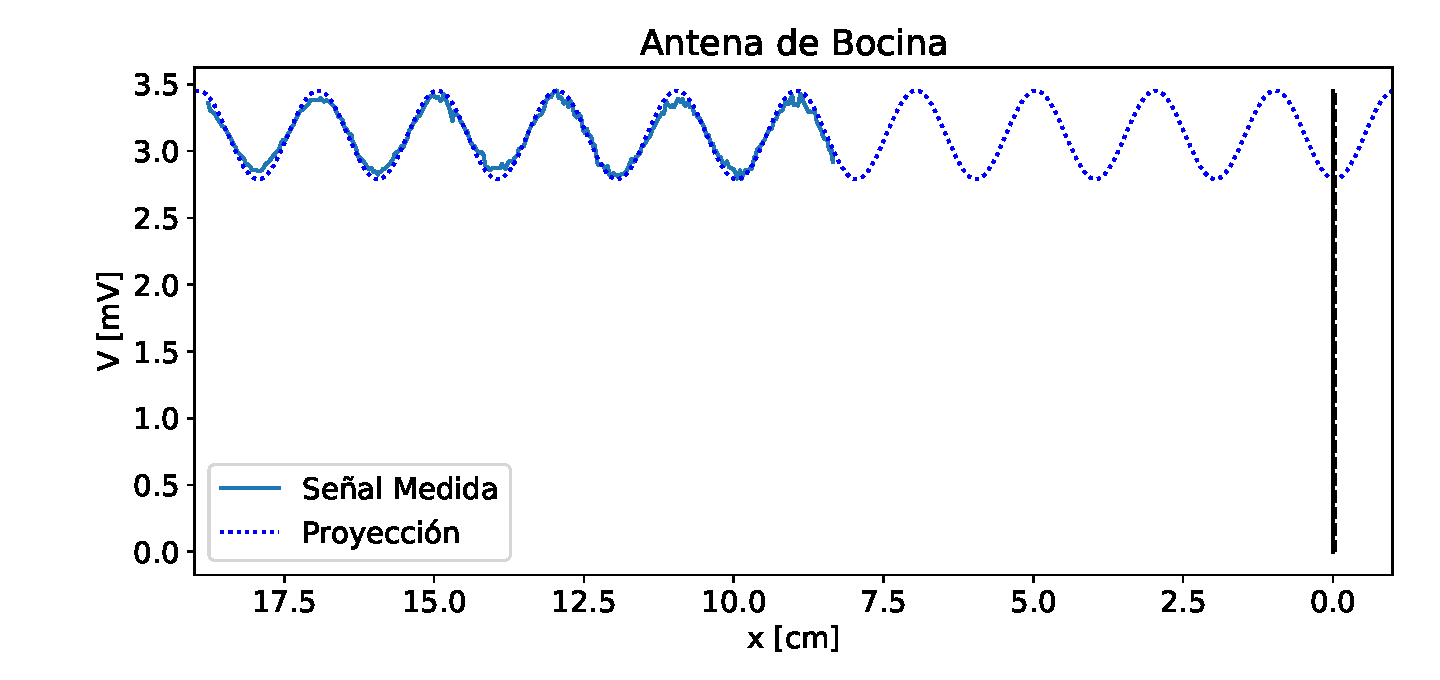
\includegraphics[width=\linewidth]{Images/antena_bocina.pdf}
    \caption{Perfil de la onda para el caso en que el plano de carga es una antena de bocina. En azul continuo se muestra la curva de los datos obtenidos, en azul punteada, la continuación analítica de la función. La línea negra vertical representa la posición del plano de carga.}
    \label{fig:bocina}
\end{figure}
Se midió un valor para el ROE de
$$
\text{ROE} = 1.24\pm?
$$
Y un valor de $\delta$ de
$$
\delta = -0.008\lambda_g
$$
\subsection{Adaptación de Impedancia con la antena detectora}
Luego de colocar el Rx a 10 cm de la antena de bocina en el plano de carga, se obtuvo un valor para la ROE de
$$
\text{ROE} = 13.3\pm?
$$
y un $\delta$ es de
$$
\delta = 0.6\lambda_g
$$
Con estos datos, utilizando el diagrama de Smith, se pudo ver que la admitancia del adaptador es de
$$
y_a = 3.4j
$$
y que la distancia del plano de carga al adaptador es
$$
\ell = 7.8 \text{ cm}
$$
Por último, se tuvo que fijar con qué profundidad habia que insertar el adaptador en la guía de onda,
$$
s = ?
$$
Se presenta en la figura x, el perfil de la onda desadaptada en contraste con el perfil de la onda adaptada,
\\ \\
fig 
\\ \\
Y, en la Figura x, se grafica el voltaje medido por la antena con la guía desadaptada, en contraste con el voltaje medido por la guía adaptada,
\\ \\
fig
\\ \\
\section{Discusión}
Se ve que el ROE para el caso de la placa de cobre en el plano de carga es tres ordenes de magnitud mayor que el ROE para el caso del aire. Esto se debe a que el caso de la placa de metal, asemeja un corto circuito, por lo tanto hay mayor reflexión para el caso del aire, que asemeja un circuito abierto. \\ \\
También se ve que, el ROE de valor más bajo fue para el caso de la corneta. Esto se debe a que, por la forma que tiene ésta, la onda se ve disipada al salir de la guía, similar a una placa acústica, y por eso la corneta es el caso mejor adaptado de los tres. \\ \\
Se observa además, que el ROE de la onda cuando la antena receptora se encuentra a continuación del plano de carga, es mayor que el ROE de la onda cuando ésta no se encuentra colocada. Esto quiere decir, que el hecho de colocar la antena produce una reflexión de la señal, y esta se ve reflejada dentro de la guía. \\ \\
Se puede notar que, luego de la adaptación de la guía con la antena detectora colocada, una disminución en el ROE, indicando que la adaptación fue exitosa. Además, el voltaje medido por la antena, se ve incrementado luego de la adaptación, o sea que mayor señal está siendo transmitida, como era de esperar.
\section{Conclusiones}

Se caracterizó una guía de ondas electromagnéticas rectangular, cuya fuente de ondas era un diodo Gunn. Se obtuvieron los siguientes valores. Para la frecuencia $f$ de trabajo del diodo,
$$
f=(10.53\pm 0.05) \text{ GHz}
$$
Para la longitud de onda $\lambda_g$ de la onda dentro de la guia,
$$
\lambda_g = (3.97\pm ) \text{ cm}
$$
Y una impedancia característica $Z_0$ de
$$
Z_0 = (525.6 \pm ) \text{ } \Omega
$$
Luego se pasó a analizar la onda estacionaria formada dentro de la onda debido a distintos planos de carga, como aire, una placa de cobre, y una bocina. Esto se hizo para luego proceder a adaptar la impedancia de la guía, observando con una antena receptora, que la señal que se transmite es mayor cuando el sistema se encuentra adaptado, que cuando está adaptado. \\ \\
Luego de la adaptación de impedancia, se vio una disminución en el cociente entre las amplitudes máximas y mínimas de la onda. Además, se vió un incremento en la señal que se transmitía por la guía. Debido a esto, se concluye que la adaptación de impedancias fue exitosa. \\ \\


\bibliography{LockIn}
\bibliographystyle{unsrt}

\end{multicols}
\newpage
\begin{appendices}
\vspace{-1em}
\hrule
\vspace{1em}
\normalsize
\section{Apéndice 1 - Resolución Numérica con Python}
\begin{multicols}{2}
    Se registra un vector de mediciones experimentales de la onda estacionaria \texttt{[x, v]}, de estos datos se extraen

    \begin{equation*}
        \mathtt{vmax} = \mathtt{max(v)} \qquad \qquad \mathtt{vmin} = \mathtt{min(v)}
    \end{equation*}\\[-1em]

    Los datos se ajustan a la función \ref{eq:fit} que aproxima el perfil de la onda estacionaria, de carácter $\frac{\lambda_g}{2}$-periódico.

    \begin{equation}\label{eq:fit}
        \mathtt v = A_0 -A\cos(2k\mathtt x-\phi)
    \end{equation}\\[-1em]

    Donde $A$ y $A_0$ se calculan a partir de \texttt{vmax} y \texttt{vmin}, y $k = \frac{2\pi}{\lambda_g}$, dejando a $\phi$ como parámetro de ajuste.\\

    A partir de estos datos se calculan la razón de onda estacionaria y el desplazamiento del plano de carga

    \begin{equation*}
        \mathrm{ROE} = \frac{\mathtt{vmax}}{\mathtt{vmin}}\qquad\qquad\delta = \frac{\phi}{2\pi}\,\frac{\lambda_g}{2}
    \end{equation*}\\[-1em]

    Notar que el valor de $\mathtt{x} = \delta$ es el que minimiza la función de ajuste \ref{eq:fit}. A continuación el procedimiento es equivalente al procedimiento gráfico realizado con el diagrama de Smith, presentado en el Apéndice 2.\\

    A partir de la ROE y $\delta$, se calcula el coeficiente de reflexión $\Gamma = \left|\Gamma\right|e^{j\phi_\Gamma}$ a partir de su módulo y fase

    \begin{equation*}
        \left|\Gamma\right| = \frac{\mathrm{ROE}-1}{\mathrm{ROE}+1}\qquad\qquad \phi_\Gamma = \pi-2k\delta
    \end{equation*}\\[-1em]

    \begin{figure}[H]
        \centering
        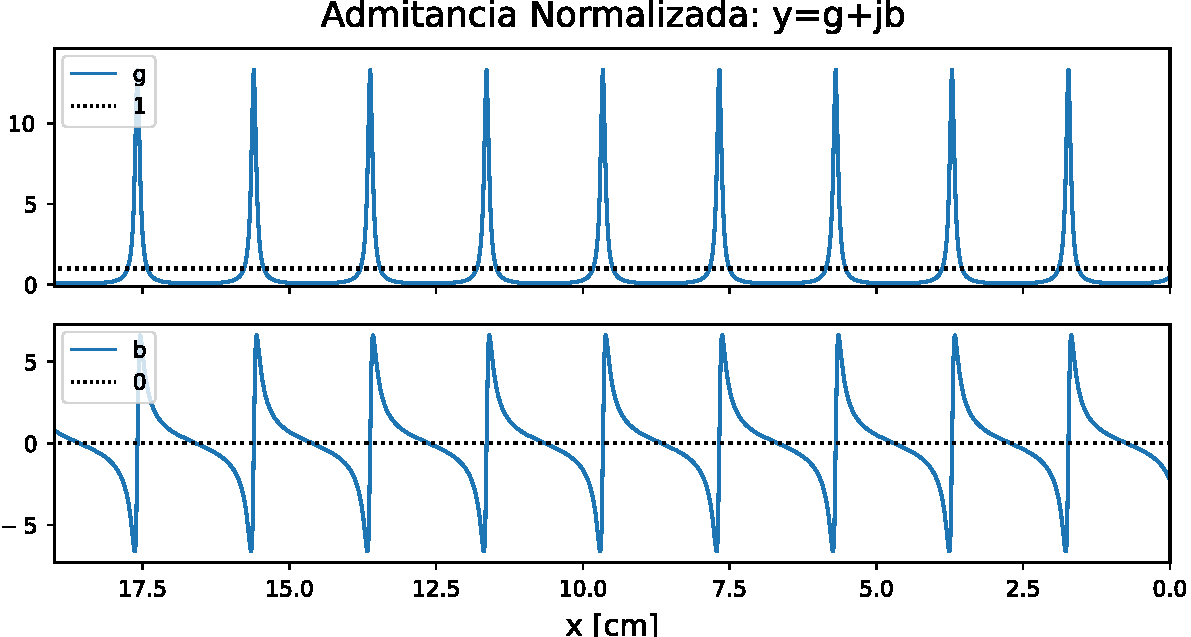
\includegraphics[width=\linewidth]{Images/ydex.pdf}
        \caption{Gráfico superior: Conductancia normalizada y recta $g=1$, intersecciones con la recta $g=1$ son candidatos a adaptacion de impedancia.
            Gráfico inferior: Suceptancia normalizada y recta $b=0$, suceptancias negativas son inductivas y suceptancias positivas son capacitivas.}
        \label{fig:ydex}
    \end{figure}
    Teniendo el valor de $\Gamma$ se expresa la admitancia normalizada en función de la distancia al plano de carga a partir de la ecuación \ref{eq:y_normal}. La admitancia se grafica en su parte real e imaginaria y se presenta en la figura \ref{fig:ydex}\\

    Se define un margen de tolerancia $\epsilon = 0.01$\footnote{Se define un márgen de tolerancia debido al error de discretización}, y se itera sobre los índices \texttt{i} de \texttt{y}, seleccionando aquellos que cumplen las siguientes condiciones

    \begin{itemize}
        \item La conductancia normalizada es igual a 1 dentro del margen de tolerancia
        $$\mathtt{ 1-\epsilon \le np.real(y[i]) \le  1+\epsilon}$$
        \item Debido a que el stub en paralelo es capacitivo, la suceptancia en la guía necesita ser inductiva
        $$\mathtt{np.imag(y[i])< 0}$$
    \end{itemize}

    A partir de los índices \texttt{i} que cumplen estas dos condiciones simultaneamente se obtienen la posición $\ell$ del adaptador capacitivo y la admitancia de este $y_a$ 
    
    \begin{equation*}
        \mathtt{\ell = x[i]\qquad\qquad y_a = - np.imag(y[i])}
    \end{equation*}\\[-1em]

    Se informan el valor de $y_a$ y los posibles valores que puede tomar $\ell$, estos además se grafican junto a la admitancia normalizada en la figura \ref{fig:ydex_l}\\

    \begin{figure}[H]
        \centering
        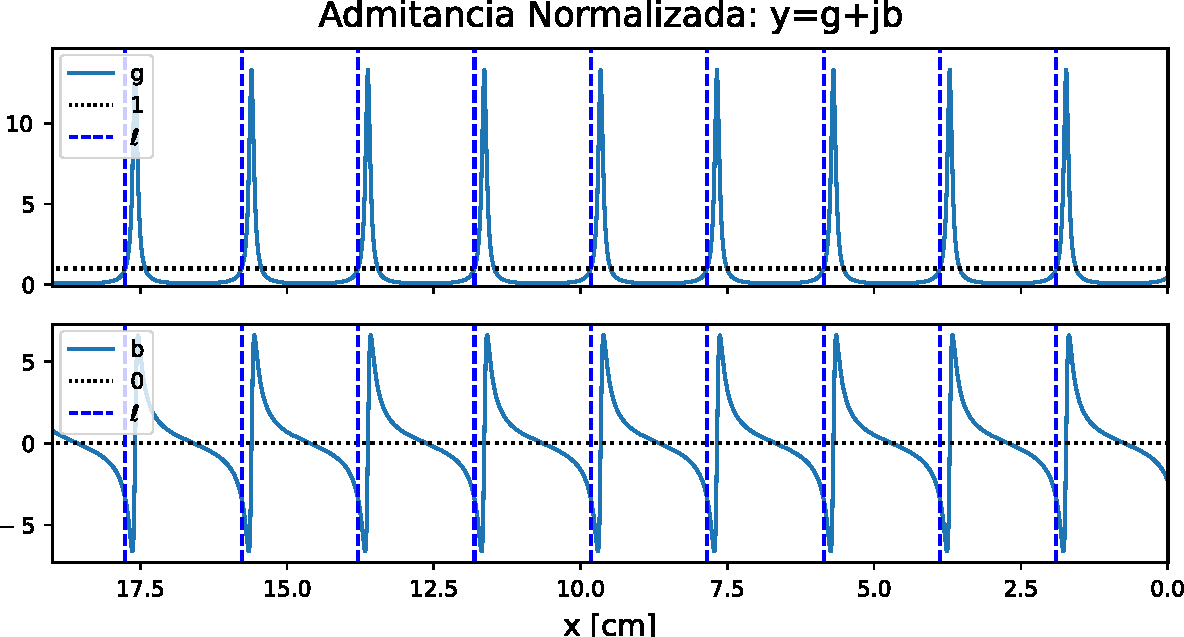
\includegraphics[width=\linewidth]{Images/ydex_l.pdf}
        \caption{Gráfico \ref{fig:ydex} argegando en línea punteada vertical las posibles ubicaciones en la guía que puede tomar un adaptador de impedancias capacitivo.}
        \label{fig:ydex_l}
    \end{figure}

\end{multicols}
\pagebreak

\end{appendices}


\begin{multicols}{2}

\end{multicols}

\end{document}